\chapter{Experimental Setup and Results}

In this chapter, I will describe our experimental setup and results. It includes a breif discussion of our optical tables setup (\ref{exp:laser-table} and \ref{exp:machine-table}), the implementation, optimization and performance of each steps (\ref{exp:zeeman}, \ref{exp:mot}, \ref{exp:gm}, \ref{exp:pump}, \ref{exp:mt} and \ref{exp:odt}) and finally some basic characteristic of our BEC (\ref{exp:bec}).

\section{Laser System}\label{exp:laser-table}
\begin{figure}
  \begin{center}
    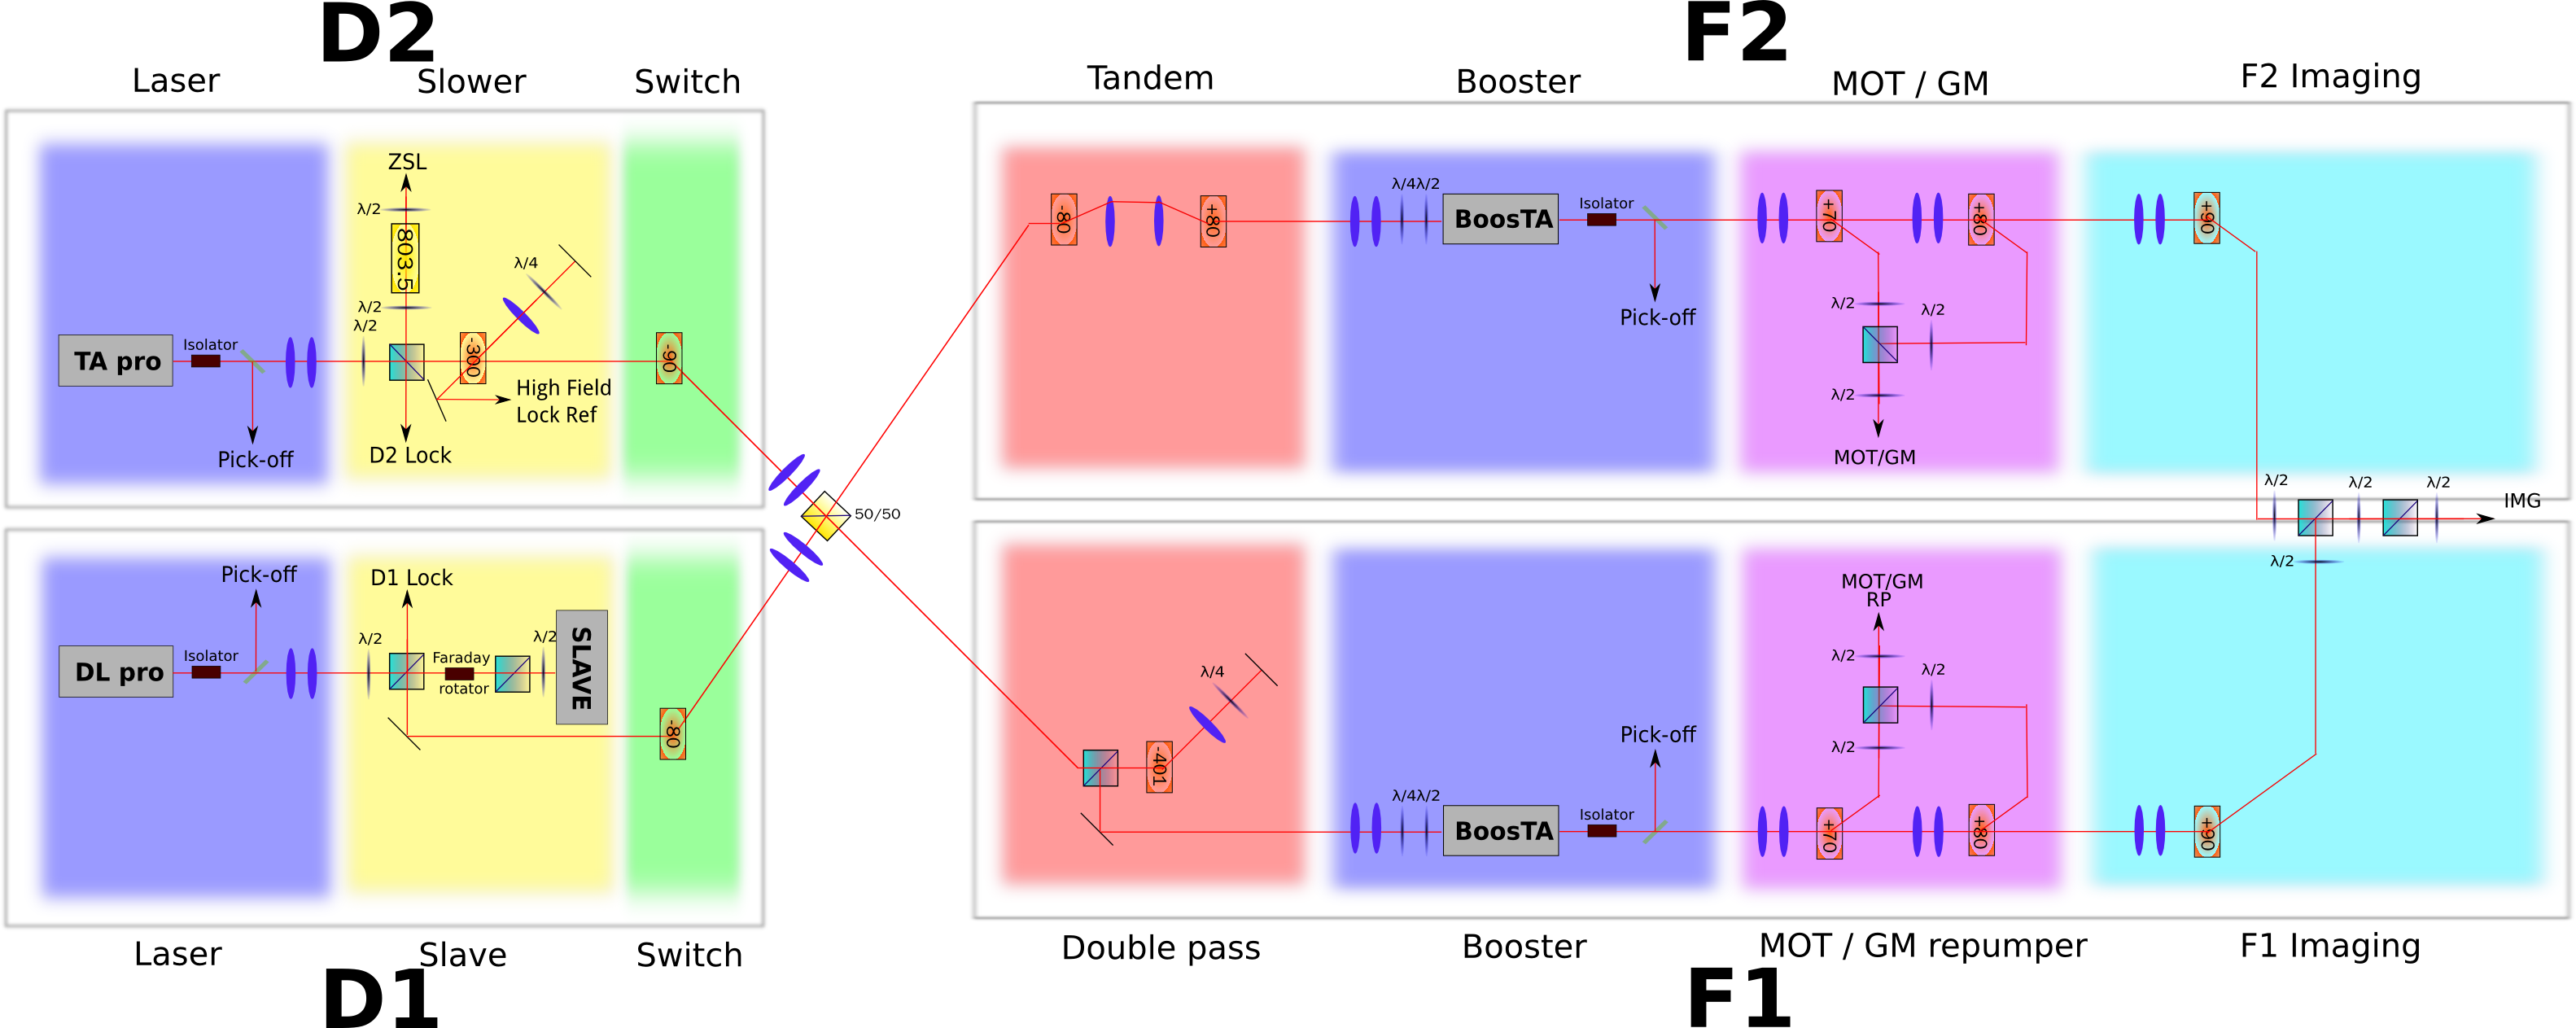
\includegraphics[width=14cm]{laser_table.png}
  \end{center}
  \caption{Schematic of the laser table design}
  \label{exp:laser-table-design}
\end{figure}

\section{Vacuum Chamber and Main Coils Configuration}\label{exp:machine-table}

\section{Spin Flip Zeeman Slower}\label{exp:zeeman}

\section{Magneto-Optical Trap (MOT) and Compressed-MOT}\label{exp:mot}

CMOT

\section{Gray Molasses}\label{exp:gm}

\section{Dark State Pumping}\label{exp:pump}

At the end of Laser cooling, the atoms are distributed in different ground states.\\
In order to trap in MT, need to go to 2, 2 / 2, 1 which are the only trappable states at both low field and high field.\\
Choose 2, 2 because we can use dark state pumping which ...

Dark State pumping with D1 light

Re-scattering, detuning

\section{Static Magnetic Trap}\label{exp:mt}

\section{Optical Dipole Trap}\label{exp:odt}

\section{Bose-Einstein Condensate}\label{exp:bec}
